% ============================================================
% Research Proposal - Bar Mordechai Damri
% Ben-Gurion University of the Negev
% Supervisors: Prof. Roni Stern, Prof. Rami Puzis
% Compile: xelatex research_proposal.tex -> bibtex research_proposal -> xelatex x2
% ============================================================

\documentclass[12pt,a4paper]{article}

\usepackage{fontspec}
\usepackage{polyglossia}
\setmainlanguage{english}
\setotherlanguage{hebrew}
\newfontfamily\hebrewfont[Script=Hebrew,BoldFont=Arial Hebrew Bold]{Arial Hebrew}

\usepackage{geometry}
\geometry{a4paper, left=2.5cm, right=2.5cm, top=2.3cm, bottom=2.5cm}

\usepackage{microtype}
\usepackage{setspace}
\setstretch{1.5}

\usepackage{xcolor}
\definecolor{bgunavy}{RGB}{27,61,110}
\usepackage{titlesec}
\titleformat{\section}{\large\bfseries\color{bgunavy}}{\thesection.}{0.6em}{}
\titleformat{\subsection}{\normalsize\bfseries\color{bgunavy}}{\thesubsection}{0.5em}{}
\titleformat{\subsubsection}{\normalsize\bfseries\itshape}{\thesubsubsection}{0.5em}{}
\titlespacing*{\section}{0pt}{10pt}{3pt}
\titlespacing*{\subsection}{0pt}{7pt}{2pt}
\titlespacing*{\subsubsection}{0pt}{5pt}{1pt}

\usepackage{amsmath}
\usepackage{amssymb}
\usepackage{booktabs}
\usepackage{tabularx}
\usepackage{enumitem}
\setlist[itemize]{topsep=2pt,itemsep=1pt,parsep=0pt,leftmargin=1.3em}
\setlist[enumerate]{topsep=2pt,itemsep=1pt,parsep=0pt,leftmargin=1.6em}

\usepackage{hyperref}
\hypersetup{colorlinks=true, linkcolor=bgunavy, citecolor=bgunavy, urlcolor=bgunavy,
  pdftitle={Research Proposal - Bar Mordechai Damri}, pdfauthor={Bar Mordechai Damri}}

\setlength{\parindent}{0pt}
\setlength{\parskip}{4pt}

\usepackage{float}
\usepackage{caption}
\usepackage{subcaption}
\captionsetup{font=small, labelfont=bf, skip=3pt}
\usepackage{multicol}
\setlength{\columnsep}{18pt}
\usepackage{graphicx}
\graphicspath{{figures/}}
\usepackage{colortbl}
\usepackage{algorithm}
\usepackage{algpseudocode}
\usepackage[round]{natbib}
\setlength{\bibsep}{2pt}

\newcommand{\dist}{d}
\newcommand{\simf}{\mathrm{sim}}

\begin{document}

% ============================================================
% COVER PAGE
% ============================================================
\begin{titlepage}
\centering\singlespacing
\vspace*{0.1cm}

\includegraphics[height=2.1cm]{bgu_logo.png}\\[10pt]
{\large\bfseries Ben-Gurion University of the Negev}\\[5pt]
{\normalsize The Stein Faculty of Computer and Information Science}\\[3pt]
{\normalsize The Institute for the Foundations of Artificial Intelligence}

\vspace{2.0cm}
{\LARGE\bfseries\color{bgunavy}\setstretch{1.2}
Embedding Geometric Heuristics for\\
Improving Retrieval-Augmented Generation
}

\vspace{0.8cm}
\begin{otherlanguage*}{hebrew}
{\Large\bfseries\setstretch{1.3}
הטמעת יוריסטיקות גיאומטריות לשיפור מערכות יצירה מועצמת על ידי שליפה \textenglish{\LR{(RAG):}}\\[4pt]
חקירת השפעת מבנה המרחב הווקטורי על איכות התשובה
}
\end{otherlanguage*}

\vspace{1.6cm}
{\large\itshape Research proposal}

\vspace{1.8cm}
{\large\bfseries Bar Mordechai Damri \,\texthebrew{בר מרדכי דמרי}}\\[6pt]
{\normalsize Student ID: 208915751}

\vspace{1.6cm}
{\normalsize Supervisors:}\\[8pt]
{\large\bfseries Prof. Roni Stern \quad Prof. Rami Puzis}

\vfill
\end{titlepage}

% ============================================================
% ABSTRACT
% ============================================================
\setcounter{page}{2}
\section*{Abstract}

Retrieval-Augmented Generation (RAG) grounds large language model (LLM) answers in retrieved documents, so answer quality is bounded by whether retrieval recovers the ground-truth (GT) document. Dense retrievers rank documents by cosine distance to the query embedding, implicitly assuming that queries and their relevant documents occupy the same region of the embedding space. This research studies the geometric structure of the query-document embedding space in RAG and, as its overarching goal, develops geometric heuristics that exploit this structure to improve retrieval. It has three goals: (1) characterize the geometry of the space and explain why query-centric retrieval fails for a non-trivial fraction of queries; (2) develop and evaluate geometric retrieval heuristics that relocate the search anchor in the space - centroid-based anchoring, adaptive anchor updates, and document-space anchors such as hypothetical documents (HyDE) - where auxiliary signals such as LLM relevance judgments serve as instruments within the heuristics, not as the object of study; and (3) test whether the findings generalize beyond the testbed. The biomedical corpus we use is a measurement testbed, chosen because the query-document gap is most pronounced there and because prior RAG research on this domain \citep{xiong2024medrag} provides a basis for comparison; the geometric constructions we employ (neighborhood circles, the query-centroid-ground-truth triangle) are likewise means of probing the space, not research goals.

\begin{otherlanguage*}{hebrew}\sloppy
\subsection*{\texthebrew{תקציר}}
מערכות יצירה מועצמת על ידי שליפה \textenglish{\LR{(RAG)}} מבססות את תשובות מודל השפה על מסמכים שנשלפו, ולכן איכות התשובה מוגבלת ביכולת שלב השליפה למצוא את מסמך האמת \textenglish{\LR{(GT)}}. מנגנוני שליפה צפופים מדרגים מסמכים לפי מרחק קוסינוס מהטמעת השאילתה, מתוך הנחה סמויה שהשאילתה והמסמכים הרלוונטיים לה שוכנים באותו אזור של מרחב ההטמעה. מחקר זה בוחן את המבנה הגיאומטרי של מרחב ההטמעה שאילתה-מסמך במערכות \textenglish{\LR{RAG}}, ומטרת-העל שלו היא פיתוח יוריסטיקות גיאומטריות המנצלות מבנה זה לשיפור השליפה. למחקר שלוש מטרות: (1) לאפיין את הגיאומטריה של המרחב ולהסביר מדוע שליפה ממוקדת-שאילתה נכשלת בחלק לא מבוטל מהשאילתות; (2) לפתח ולהעריך יוריסטיקות שליפה גיאומטריות המזיזות את עוגן החיפוש במרחב, כגון עיגון מבוסס-צנטרואיד, עדכון אדפטיבי של העוגן ועוגנים במרחב המסמכים (למשל מסמכים היפותטיים, \textenglish{\LR{HyDE}}), כאשר שיפוטי רלוונטיות של מודל שפה משמשים רק ככלי עזר בתוך היוריסטיקות; (3) לבדוק אם הממצאים תקפים גם מחוץ לסביבת הניסוי. הקורפוס הביו-רפואי שבו אנו משתמשים הוא סביבת מדידה, שנבחרה משום שהפער בין שאילתות למסמכים בולט בה במיוחד ומשום שמחקר \textenglish{\LR{RAG}} קודם בתחום זה מספק בסיס להשוואה. אף המבנים הגיאומטריים שבהם אנו משתמשים (מעגלי שכנות, משולש שאילתה-צנטרואיד-מסמך אמת) הם אמצעים לחקירת המרחב ולא מושא המחקר.
\end{otherlanguage*}

% ============================================================
% 1. BACKGROUND
% ============================================================
\section{Scientific background}
\label{sec:background}

\subsection{Retrieval-augmented generation: pipelines and where they fail}

RAG decouples knowledge storage from language modeling: at inference time, documents are retrieved from an external corpus and given to the LLM as context \citep{lewis2020rag}. The design space has grown considerably since. Fusion-in-Decoder reads many retrieved passages independently and fuses them in the decoder \citep{izacard2021fid}; RETRO retrieves token chunks from a trillion-token corpus inside the model \citep{borgeaud2022retro}; in-context RALM simply prepends retrieved documents to a frozen LLM and still obtains large gains \citep{ram2023ralm}. A recent survey organizes this landscape into naive, advanced, and modular RAG \citep{gao2023ragsurvey}. A second line of work decides \emph{when} and \emph{how often} to retrieve rather than \emph{what}: FLARE retrieves whenever the upcoming sentence has low-confidence tokens \citep{jiang2023flare}; IRCoT interleaves retrieval with chain-of-thought steps \citep{trivedi2023ircot}; Self-RAG trains the LLM to decide to retrieve and to critique what it retrieved \citep{asai2024selfrag}; Adaptive-RAG routes queries by predicted complexity \citep{jeong2024adaptiverag}; Corrective RAG evaluates retrieved documents and falls back to web search when they look wrong \citep{yan2024crag}; GraphRAG replaces passage retrieval by community summaries over an entity graph for corpus-wide questions \citep{edge2024graphrag}.

Across all of these designs, the generator cannot repair a retrieval miss. If the GT document is not retrieved, the LLM cannot produce a correct grounded answer, and irrelevant context actively degrades it \citep{shi2023distractors}; even when the right document is present, its position in the context matters \citep{liu2024lost}. Retrieval quality therefore bounds RAG quality, which is why the retrieval step is the object of this research.

\subsection{Finding relevant documents: the state of the art}
\label{sec:sota}

\textbf{Dense first-stage retrieval.} The dominant retriever is a bi-encoder that maps queries and documents independently into one vector space and ranks by embedding similarity \citep{karpukhin2020dpr}; \citet{zhao2024densesurvey} survey the field. Its quality is driven by training: contrastive pre-training without labels \citep{izacard2022contriever}, weakly-supervised pairs at web scale \citep{wang2022e5}, task instructions embedded with the text \citep{su2023instructor}, and better negatives - cross-batch and denoised hard negatives \citep{qu2021rocketqa}, negatives mined from the model's own nearest neighbors \citep{xiong2021ance}, and optimized hard-negative training \citep{zhan2021hardneg}. All of these change the encoder; the search itself remains nearest-neighbor search from the encoded query.

\textbf{Richer scoring functions.} Late-interaction models keep one vector per token and score with MaxSim \citep{khattab2020colbert,santhanam2022colbertv2}; learned sparse models such as SPLADE expand queries and documents in vocabulary space and use an inverted index \citep{formal2021splade}. \citet{luan2021sparse} show analytically why a single fixed-size query vector has limited capacity and propose multi-vector and hybrid scoring as the remedy. These methods change \emph{how} a candidate is scored against the query representation, not \emph{where} in the space the search is anchored.

\textbf{Re-ranking.} A cross-encoder or an LLM re-scores a candidate list produced by a first-stage retriever: monoT5 generates a relevance token \citep{nogueira2020monot5}; RankGPT re-ranks listwise with an instructed LLM and distills the ability into small models \citep{sun2023rankgpt}. LLMs are also used as relevance \emph{judges} that produce graded labels agreeing well with searcher preferences \citep{thomas2024llmjudge}. Re-rankers can only permute the candidates they are given; a document the first stage missed stays missed.

\textbf{Query rewriting and expansion.} Query2doc prompts an LLM for a pseudo-document and appends it to the query \citep{wang2023query2doc}; Rewrite-Retrieve-Read trains a rewriter from reader feedback \citep{ma2023rewrite}; HyDE embeds an LLM-written hypothetical answer and retrieves with that embedding, which lies in ``document space'' \citep{gao2023hyde}. Its authors acknowledge that the generated document may contain false details and argue that the encoder's dense bottleneck filters them out; whether this holds in biomedicine, where precise facts matter, is what our Hypothesis~D tests.

\textbf{Relevance feedback.} Pseudo-relevance feedback (PRF) assumes the top-ranked documents are relevant and reformulates the query from them, classically with the Rocchio update that moves the query vector toward their centroid \citep{rocchio1971relevance}. In dense retrieval, vector PRF averages or Rocchio-combines the top-$k$ embeddings with the query embedding and works best when the query keeps most of the weight and only a few feedback documents are used \citep{li2023vectorprf}; its benefit extends to LLM-based dense retrievers \citep{li2025llmvprf} and can close much of the gap between small and large retrievers \citep{prfllm2026}. ColBERT-PRF does the same at the token-embedding level \citep{wang2023colbertprf}, ANCE-PRF learns a query encoder that reads the query together with its top-ranked documents \citep{mao2021anceprf}, and the Rocchio update has been made robust to position bias when the feedback comes from clicks \citep{li2022corocchio}. The shared weakness is that irrelevant top-ranked documents contaminate the feedback, and the damage grows as the first-stage ranking gets worse \citep{li2022prfquality}. Generative relevance feedback replaces the retrieved feedback documents by LLM-written text \citep{mackie2023grf,mackie2023grfdense,zhang2024mugi}, or steers the generation with sentences taken from the corpus \citep{lei2024csqe}.

\textbf{The biomedical setting.} Out of domain, dense retrievers often underperform even BM25, including on biomedical collections \citep{thakur2021beir}. In biomedical QA, short expert-written questions must be matched against dense scientific abstracts \citep{tsatsaronis2015bioasq}. Domain pre-training such as BioBERT \citep{lee2020biobert} improves biomedical language understanding but does not by itself train the encoder to place questions near their answer documents; that requires dedicated retrieval training \citep{jin2023medcpt}. Benchmarks of RAG for medicine exist and provide a basis for comparison \citep{xiong2024medrag}. This is why we use a biomedical corpus as our testbed: the gap is most pronounced, and thus most measurable, there.

\subsection{Moving the search anchor at test time}
\label{sec:anchor-lit}

A smaller body of work moves the query representation itself at inference time, which is the operation this proposal studies. TOUR optimizes the query embedding by gradient descent against pseudo-labels from a cross-encoder re-ranker and shows that this generalizes the Rocchio update \citep{sung2023tour}. ReDE-RF asks an LLM which of the first-pass documents are relevant and then searches from the embeddings of those real documents instead of from a hypothetical one, arguing that judging relevance is easier for the LLM than generating domain knowledge \citep{jataria2024rederf}. BAGEL treats passage retrieval under an LLM budget as a global optimization problem: it fits a query-specific Gaussian process over the embedding space from sparse LLM relevance scores and selects the next passages to score by balancing exploitation and exploration \citep{bagel2026}. Embedding surgery edits selected \emph{document} embeddings at query time from editorial, click, or LLM feedback \citep{embsurgery2026}. On the generation side, Iter-RetGen alternates retrieval and generation so that each draft answer becomes the next retrieval query \citep{shao2023iterretgen}, and a recent survey organizes this growing family under the heading of test-time corpus feedback \citep{feedback2025survey}.

These works establish that relocating the anchor with LLM feedback is a live and productive direction, and several of them are natural baselines for this research. What none of them provides is a measurement of \emph{where} the relevant documents and the ground truth sit relative to the query and to each other. Each chooses its update rule a priori (a gradient step, a replacement of the query by selected documents, a Gaussian-process posterior) rather than deriving it from the observed geometry of the query's neighborhood, and none reports whether the anchor should move all the way to the relevant cluster or only part of the way. Section~\ref{sec:prelim} shows that this distinction matters: replacing the query by the centroid of confirmed-relevant documents is strongly harmful on our testbed, while a small pull toward it helps.

\subsection{Measuring relevance: LLM judges and their limits}
\label{sec:judges}

Any method that uses relevance feedback at test time, and any evaluation of retrieval, depends on relevance labels. LLMs are now used as relevance assessors at scale: with careful prompting their labels agree with searchers' preferences about as well as human assessors do \citep{thomas2024llmjudge}, and the open-source reproduction UMBRELA correlates highly with human judgments across the TREC Deep Learning tracks \citep{upadhyay2024umbrela}. In the TREC 2024 RAG track, system rankings induced by UMBRELA labels correlated highly with those from fully manual assessment \citep{upadhyay2024trecrag}. The limits are documented as well: LLM judges are sensitive to prompt wording, can be gamed by systems that optimize against them, and are more lenient than human assessors \citep{soboroff2024cantreplace,rahmani2025benchmarking}; the LLMJudge collection was released to study these biases systematically \citep{rahmani2025llmjudge}. Two consequences shape this proposal. First, LLM judgments are reliable enough to serve as an \emph{instrument}, and the preliminary results confirm that on our testbed they are geometrically consistent (Section~\ref{sec:prelim}). Second, graded labels expose a problem that binary ground truth hides: a query often has several fully relevant documents, so an evaluation that counts only the single labeled GT understates retrieval quality. Standard retrieval metrics (recall@$k$, MRR, nDCG) and RAG evaluation frameworks \citep{yu2025rageval} assume the relevant set is known; we therefore report exact-GT and soft-success measures side by side.

\subsection{What these methods do not account for}

Table~\ref{tab:families} groups the methods above by what they change. Four families leave the anchor where it is: better encoders, richer scoring, re-ordering of a fixed candidate list, and control of when to retrieve. Two move it. Query rewriting moves the search anchor as a by-product of text generation: the new anchor is wherever the rewritten text happens to embed, chosen without reference to where the relevant documents lie. PRF and the test-time feedback methods of Section~\ref{sec:anchor-lit} move the anchor in vector space on purpose, but each applies a fixed update rule - trust the top-$k$, take a gradient step, replace the query by the selected documents - and, as our results in Section~\ref{sec:prelim} show, replacing the query is harmful when relevant and irrelevant documents are interleaved near it. None of these methods measure the local geometry of the query's neighborhood - the direction from the query to the cluster of relevant documents, the distance between them, or the offset of the GT from that cluster - and none derive the size of the anchor's move from such measurements. That is the gap this research addresses.

\begin{table}[H]
\centering\small
\caption{Families of retrieval methods and the mechanism each one changes. ``Anchor'' is the point in embedding space from which nearest-neighbor search is run.}
\label{tab:families}
\setstretch{1.05}
\begin{tabularx}{\textwidth}{>{\raggedright\arraybackslash}p{2.7cm}>{\raggedright\arraybackslash}X>{\raggedright\arraybackslash}p{3.4cm}>{\raggedright\arraybackslash}p{3.1cm}}
\toprule
Family & Representative methods & Moves the anchor? & Uses neighborhood geometry? \\
\midrule
Encoder training & DPR, Contriever, E5, INSTRUCTOR, RocketQA, ANCE & no & no \\
Scoring function & ColBERT, SPLADE, multi-vector hybrids & no & no \\
Re-ranking & monoT5, RankGPT, LLM judges & no (permutes candidates) & no \\
Retrieval control & FLARE, IRCoT, Self-RAG, Adaptive-RAG, CRAG & no & no \\
Query rewriting & Query2doc, Rewrite-Retrieve-Read, HyDE & yes, via generated text & no \\
Relevance feedback & Rocchio, vector PRF, ColBERT-PRF, ANCE-PRF & yes, toward top-$k$ & only the top-$k$ mean \\
Test-time anchor updates & TOUR, ReDE-RF, BAGEL, embedding surgery & yes, by a fixed rule & indirectly (no measurement) \\
\midrule
\textbf{This proposal} & geometric anchoring & yes, by measured geometry & yes \\
\bottomrule
\end{tabularx}
\end{table}

\subsection{The geometry of embedding spaces}

\textbf{Anisotropy.} Contextual embedding spaces are strongly anisotropic: representations concentrate in narrow cones, which compresses cosine similarities and reduces their discriminative power \citep{ethayarajh2019contextual}. The phenomenon was first described for generation models as representation degeneration \citep{gao2019degeneration}; a handful of rogue dimensions can dominate cosine similarity \citep{timkey2021rogue}. Post-processing remedies remove the common mean and top principal components \citep{mu2018allbutthetop}, map the space to an isotropic Gaussian \citep{li2020bertflow}, or whiten it \citep{su2021whitening}; the same anisotropy has been measured in the query and document representations of dense retrievers, where isotropization improves retrieval \citep{jung2023isotropic}.

\textbf{Training-objective geometry.} \citet{wang2020alignment} characterize contrastive representations on the hypersphere by alignment of positive pairs and uniformity of the overall distribution; SimCSE shows that contrastive fine-tuning improves uniformity of sentence embeddings \citep{gao2021simcse}, while contrastive objectives can also suffer dimensional collapse \citep{jing2022collapse}. The retrievers in Section~\ref{sec:sota} inherit these properties, since they are all trained contrastively.

\textbf{Hubness, dimensionality, and the limits of cosine.} In high dimensions some points become hubs that are nearest neighbors of many others \citep{radovanovic2010hubs}; sentence-embedding spaces exhibit this hubness, and neighborhood quality improves when it is reduced \citep{lanzen2023hubness}. For dense retrieval, false positives grow with index size at fixed dimensionality \citep{reimers2021curse}, and the fidelity of single-vector inner-product retrieval is bounded by the embedding dimension \citep{luan2021sparse}. \citet{steck2024cosine} show that cosine similarity between learned embeddings can be arbitrary, depending on how the model was regularized, and isotropy itself is in tension with the cluster structure that retrieval relies on \citep{mickus2024isotropy}. Two recent lines are closer to our per-query view: dimension importance estimation argues that the documents relevant to a query lie on a query-dependent low-dimensional manifold and re-weights embedding dimensions per query, using pseudo-relevant or pseudo-irrelevant documents \citep{faggioli2024dime,eclipse2024}; and dense query-performance prediction uses the coherence of a query's top-ranked embeddings to predict whether the query will fail \citep{vlachou2023coherence}, which is the task of Phase~1 with different features.

\textbf{Query-document asymmetry and failure analyses.} Dual encoders may share or separate the query and document towers, and the choice affects how the two populations are placed in the space \citep{dong2022dualencoder}; a recent bias-variance analysis shows that separate projections pay off exactly when the query distribution is rotated relative to the document distribution \citep{dualgeom2026}, and even a query-side PCA improves out-of-domain retrieval for most retriever-dataset pairs \citep{pcaquery2026}. Standard contrastive training aligns queries to documents but not documents to queries, which leaves the query side of the space loosely organized; adding the reverse objective pulls query embeddings toward the document distribution \citep{li2021dance}. In two-encoder vision-language models the analogous effect is well documented: the two modalities are embedded ``at arm's length'' from each other, a gap created by the narrow-cone initialization of each encoder and preserved by contrastive optimization \citep{liang2022modalitygap}. Dense retrievers fail systematically on simple entity-centric questions that lexical retrieval handles easily \citep{sciavolino2021entity}. Hard-negative mining is itself a geometric observation: the documents nearest to a query are frequently irrelevant, which is why they make effective training negatives \citep{xiong2021ance,zhan2021hardneg}.

\textbf{Positioning.} The geometric literature describes the space globally - its anisotropy, its hubs, its capacity - and prescribes fixes applied to every vector in the same way; the per-query lines (dimension importance, query-performance prediction) re-weight dimensions or predict failure but leave the anchor where it is; the test-time feedback methods move the anchor, but by a rule fixed in advance. To our knowledge, the \emph{relative} position of a query, the cluster of documents relevant to it, and the GT document has not been measured directly, and no retrieval method sizes its anchor update per query from such measurements. That measurement, and the heuristics it suggests, are the subject of this proposal; the methods of Section~\ref{sec:anchor-lit} are its baselines.

% ============================================================
% 2. OBJECTIVES
% ============================================================
\section{Research objectives and expected significance}

\begin{enumerate}[label=\textbf{RQ\arabic*.}, leftmargin=2.6em]
  \item \textbf{Geometry.} What is the geometric structure of the query-document embedding space in RAG systems, and how does it explain the gap between oracle-guided and query-guided retrieval? \textit{Contribution:} a characterization of the $Q$-$C$-$GT$ triangle and of the features that predict retrieval failure.
  \item \textbf{Geometric anchoring.} Can geometric heuristics that relocate the search anchor - e.g., an adaptively updated centroid of documents confirmed relevant - reach the GT more efficiently than query-only retrieval? Auxiliary signals such as LLM relevance judgments serve as instruments within the heuristic, not as its subject. \textit{Contribution:} an adaptive geometric retrieval algorithm and its cost-accuracy curve.
  \item \textbf{Document-space anchoring.} Does moving the search anchor into document space - hypothetical document generation (HyDE) being one realization - close the query-document gap, and when does it beat query-based anchoring? \textit{Contribution:} a geometric account of when document-space anchors succeed.
  \item \textbf{Generalization.} Do the geometric findings and heuristics transfer beyond the biomedical testbed - chosen for its pronounced gap and its established RAG literature - to other specialized and general-domain datasets? \textit{Contribution:} practical guidelines for when geometry-aware retrieval is worth its cost.
\end{enumerate}

\textbf{Motivation and significance.} Retrieval quality bounds every RAG answer, yet dense retrieval rests on an untested geometric assumption. Explaining where it fails gives a principled way to diagnose retrieval errors and to correct them with heuristics built on the structure of the embedding space. The heuristics are retriever-agnostic: they operate on the vectors any bi-encoder already produces, so they compose with the encoder, scoring, and re-ranking improvements of Section~\ref{sec:sota} rather than competing with them.

% ============================================================
% 3. PROPOSED RESEARCH
% ============================================================
\section{Detailed description of the proposed research}

\subsection{Working hypotheses}
\begin{itemize}
  \item[\textbf{A.}] \textbf{Queries are geometric outliers.} Query embeddings lie in sparse regions of document space, further from their relevant documents than those documents are from each other.
  \item[\textbf{B.}] \textbf{Relevance is geometrically graded around the GT.} The more relevant a document is to the query, the closer it lies to the GT, so the relevant neighborhood forms a gradient that a moving anchor can follow; LLM judgments serve only to measure relevance.
  \item[\textbf{C.}] \textbf{Adaptive geometric anchoring is more efficient.} Moving the anchor toward the centroid of documents confirmed relevant, as the search proceeds, reaches the GT after inspecting fewer documents than a static query anchor, especially for the $\sim$30\% of queries where the GT is not ranked first.
  \item[\textbf{D.}] \textbf{HyDE has a precision trade-off in biomedicine.} HyDE moves the anchor toward the right topical cluster but not necessarily toward the document holding the precise fact.
\end{itemize}

\subsection{Research design and methods}
\label{sec:methods}

\textbf{Notation.} All vectors are $\ell_2$-normalized. $\dist(x,y)=1-x\cdot y$ is cosine distance and $\simf(x,y)=x\cdot y$ cosine similarity. $Q$ is the query embedding, $\mathcal{D}$ the document pool, $GT$ the ground-truth document, and $C$ the \emph{oracle centroid}: the normalized mean of the documents the judge scores 1.0 for the query. ``Inspecting'' a document means sending it to the relevance judge.

\textbf{Phase 1 - Geometric analysis (S1).} Characterize the failing queries against the successful ones (GT offset from the $Q$-$C$ line, neighborhood density, number of relevant documents, the per-query correlation between judged relevance and distance) and fit a model that predicts failure from these geometric features, evaluated by cross-validated ROC-AUC against the dense query-performance predictors of \citet{vlachou2023coherence}. All features are already computed for the 196 testbed queries. Replicate the outlier and triangle measurements on TREC-COVID \citep{roberts2020treccovid} and MS MARCO \citep{nguyen2016msmarco}, whose human relevance judgments supply the relevant sets without any LLM judging.

\textbf{Phase 2 - HyDE (S1-S2).} For each query, generate a 3-5 sentence hypothetical biomedical passage with the judge LLM, embed it with the cached encoder, and use it as the anchor: one generation per query, 196 in total. Report accuracy and cost against B1 and against ReDE-RF \citep{jataria2024rederf}, which replaces the hypothetical document by real judged ones; locate the HyDE embedding in the $Q$-$C$-$GT$ frame; and test HyDE as the starting anchor for Phase~3.

\textbf{Phase 3 - Adaptive geometric anchoring (S1-S2).} Algorithm~\ref{alg:adaptive} is the method under development. At step $t$ the next document to inspect is chosen by
\begin{equation}
  \text{score}(d,t) = \alpha(t)\,\simf(d,Q) + \bigl(1-\alpha(t)\bigr)\,\simf(d,C_t),
  \label{eq:score}
\end{equation}
where $C_t$ is the normalized centroid of the documents judged $\geq\theta$ so far. The design decisions that distinguish it from the prototype in Section~\ref{sec:prelim-adaptive} are: (i) a \emph{schedule} $\alpha(t)$ that keeps the anchor on $Q$ until the centroid rests on enough support ($|R_t|\ge m$) and then moves it gradually; (ii) a \emph{trigger}: the anchor starts moving only after an inspected document is judged below the relevance threshold $\theta$, so queries that B1 already solves are never perturbed; (iii) \emph{repulsion}: $\alpha>1$ pushes the anchor away from a centroid of documents judged irrelevant; (iv) \emph{two stopping rules}: the first document scored 1.0 (soft success) and the GT itself (exact success), reported separately.

\begin{algorithm}[H]
\caption{Adaptive geometric anchoring (proposed; Phase 3)}
\label{alg:adaptive}
\begin{algorithmic}[1]
\Require query $Q$, pool $\mathcal{D}$, judge $J:\mathcal{D}\to[0,1]$, threshold $\theta$, minimum support $m$, schedule $\alpha(\cdot)$, budget $B$
\State $U \gets \mathcal{D}$;\; $R \gets \emptyset$;\; $N \gets \emptyset$;\; $C \gets Q$;\; triggered $\gets$ false
\For{$t = 1,\dots,B$}
  \State $a \gets$ \textbf{if} triggered \textbf{and} $|R|\ge m$ \textbf{then} $\alpha(t,|R|)$ \textbf{else} $1$
  \State $d^\ast \gets \arg\max_{d\in U}\; a\,\simf(d,Q) + (1-a)\,\simf(d,C)$ \Comment{repulsion variant: $a>1$ with $C\gets\mathrm{normalize}(\mathrm{mean}(N))$}
  \State $s \gets J(d^\ast)$;\; $U \gets U\setminus\{d^\ast\}$ \Comment{one inspection}
  \If{$s \ge \theta$} $R \gets R\cup\{d^\ast\}$;\; $C \gets \mathrm{normalize}(\mathrm{mean}(R))$ \Else\ $N \gets N\cup\{d^\ast\}$;\; triggered $\gets$ true \EndIf
  \If{$s = 1.0$} record soft success at step $t$ \EndIf
  \If{$d^\ast = GT$} \Return $t$ \Comment{exact success: documents inspected until GT} \EndIf
\EndFor
\State \Return $B{+}1$ \Comment{GT not reached within budget}
\end{algorithmic}
\end{algorithm}

\textbf{Baselines.} Beyond B1 and the static family of Table~\ref{tab:results}, Algorithm~\ref{alg:adaptive} is compared against the published anchor-moving methods of Section~\ref{sec:anchor-lit}, re-implemented on the same offline framework: vector PRF with Rocchio weights \citep{li2023vectorprf}, ReDE-RF-style replacement of the query by LLM-selected documents \citep{jataria2024rederf}, TOUR-style gradient updates with the judge as the pseudo-labeler \citep{sung2023tour}, and LLM re-ranking of B1's top-$k$ \citep{sun2023rankgpt}. All consume the same pre-computed judgments, so the comparison is at equal inspection budget.

\textbf{Evaluation.} All algorithms are evaluated on the offline simulation framework (pre-computed embeddings and LLM scores) by: mean number of documents inspected before reaching the GT; top-1/top-10 accuracy at inspection budgets $B\in\{1,2,3,5,10\}$; a soft-success rate (first document judged fully relevant); and the full cost-accuracy curve per method against B1. Differences between methods are tested with a paired bootstrap over the 196 queries (and over the query sets of the replication collections), and every reported gain is broken down into the queries B1 solves and the queries it fails, since the two groups behave differently (Section~\ref{sec:prelim-static}). Because every judgment is pre-computed, any variant of Algorithm~\ref{alg:adaptive} is evaluated on all 196 queries in seconds, which makes a wide sweep of $\theta$, $m$, and $\alpha(\cdot)$ practical.

\textbf{Phase 4 - Generalization and publication (S2-S3).} Repeat Phases 1 and 3 on one specialized-domain and one general-domain dataset, and submit to SIGIR, ECIR, ACL, or EMNLP.

\subsection{Preliminary results}
\label{sec:prelim}

\subsubsection{Testbed and measurement instruments}

\textbf{Testbed.} 196 biomedical questions, a pool of 5,035 PubMed abstracts, 768-dimensional bi-encoder embeddings (\texttt{all-mpnet-base-v2}), and $\sim$1M query-document pairs - every query against the entire pool - scored by a Gemini-2.5-flash-lite judge on a graded scale (0.1-1.0, almost entirely six levels: 0.1, 0.2, 0.4, 0.6, 0.8, 1.0). Exhaustive judging is what makes the oracle centroid $C$ and the offline simulation possible.

\textbf{Instruments.} Four constructions are used to probe the space; they are tools, not research goals.
\begin{itemize}
  \item \emph{Relevant set} $G_3$: documents the judge scores 1.0. Its normalized mean is the oracle centroid $C$.
  \item \emph{Neighbourhood circles.} $G_1 = \{d : \dist(d,Q) \le \dist(Q,GT)\}$, the documents a query-anchored retriever must pass before reaching the GT; $G_2 = \{d : \dist(d,C) \le \dist(C,GT)\}$, the same construction anchored at $C$.
  \item \emph{The $Q$-$C$-$GT$ spherical triangle}, with vertex angles computed by the spherical law of cosines from arc lengths $\arccos(1-\dist)$, and the \emph{$Q$-$C$ coordinate frame}, which places $Q$ at $-1$, $C$ at $+1$ and records where the GT falls.
  \item \emph{Trilateration plots} (Fig.~\ref{fig:trilateration}): a 2-D rendering of one query's pool that preserves the exact cosine distances of every document to $Q$ and to $GT$, with the circles and $G_3$ overlaid.
\end{itemize}

\begin{figure}[H]
\centering
\begin{subfigure}[t]{0.49\textwidth}
  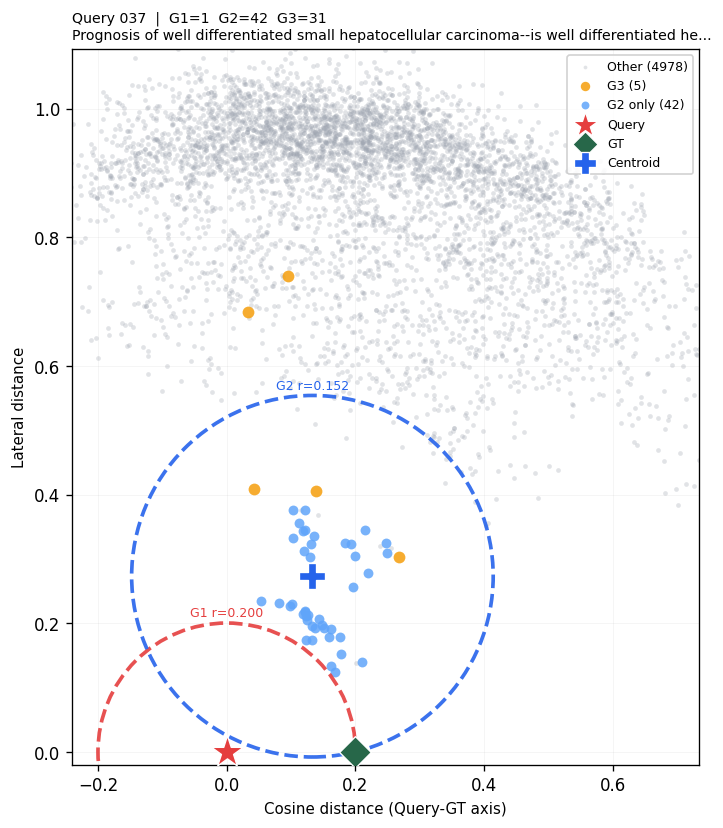
\includegraphics[width=\textwidth]{trilateration_q037.png}
  \caption{Query 37: $|G_1|=1$, $|G_2|=42$, $|G_3|=31$. The centroid $C$ sits inside a dense cloud of relevant documents that the query circle misses entirely.}
\end{subfigure}\hfill
\begin{subfigure}[t]{0.49\textwidth}
  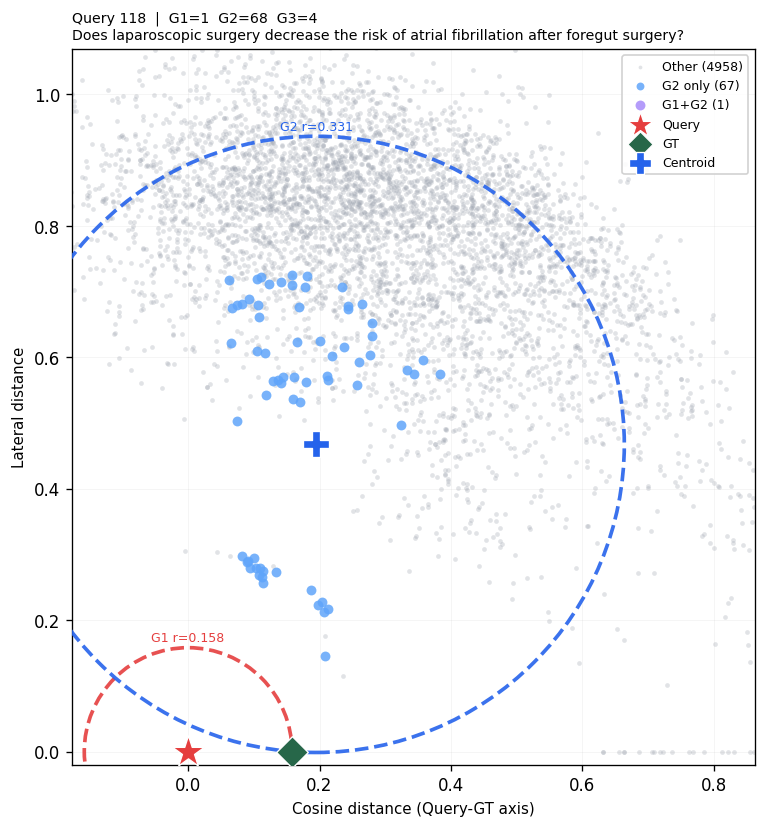
\includegraphics[width=\textwidth]{trilateration_q118.png}
  \caption{Query 118: $|G_1|=1$, $|G_2|=68$, $|G_3|=4$. Here $C$ is farther from the GT than $Q$ is, yet its circle still captures many documents: the GT's own neighborhood is dense.}
\end{subfigure}
\caption{Trilateration views of two queries. Axes are exact cosine distances along and perpendicular to the $Q$-$GT$ axis; grey points are the remaining pool, orange are $G_3$ documents, blue are documents inside the centroid circle only.}
\label{fig:trilateration}
\end{figure}

\subsubsection{Finding A: queries are geometric outliers}

Across the 196 queries the query circle $G_1$ holds on average 3.1 documents (median 1) while the centroid circle $G_2$ holds 9.7 (median 6) and the relevant set $G_3$ has 17.1 (median 18). The GT lies inside $G_1$ for 84.7\% of queries and inside $G_2$ for 85.2\%, so the two circles are equally good at containing the GT, but the centroid's neighborhood is three times denser. The density is not an artifact of the radius: random anchors placed at the same distance from the GT as $C$ capture only 0.8 documents on average. With the stricter radius $\dist(Q,GT)/2$ the query circle is empty for 100\% of queries, whereas the GT circle is empty for only 77\%.

Table~\ref{tab:groups} gives the full picture, including the split between the 138 queries B1 solves and the 58 it fails: the GT sits inside the centroid circle for 77.6\% of the failing queries, against 74.1\% for the query circle, so the centroid's neighborhood is not only denser but also at least as likely to contain the target when the query-anchored retriever misses it.

\begin{table}[H]
\centering\small
\caption{Neighborhood circles over 196 queries. $G_1$ is anchored at the query, $G_2$ at the oracle centroid, $G_3$ is the set of documents judged fully relevant; ``B1 ok'' / ``B1 failed'' split queries by whether B1 ranks the GT first. Mean Jaccard overlaps: $G_1{\cap}G_2$ 0.33, $G_2{\cap}G_3$ 0.34, $G_1{\cap}G_3$ 0.12. Random anchors placed at distance $\dist(C,GT)$ from the GT capture 0.8 documents on average.}
\label{tab:groups}
\setstretch{1.05}
\begin{tabularx}{\textwidth}{>{\raggedright\arraybackslash}p{3.3cm}>{\centering\arraybackslash}X>{\centering\arraybackslash}X>{\centering\arraybackslash}X>{\centering\arraybackslash}X>{\centering\arraybackslash}X}
\toprule
 & Mean size & Median size & GT inside, all & GT inside, B1 ok ($n{=}138$) & GT inside, B1 failed ($n{=}58$) \\
\midrule
$G_1$ query circle    & 3.1  & 1  & 84.7\% & 89.1\% & 74.1\% \\
$G_2$ centroid circle & 9.7  & 6  & 85.2\% & 88.4\% & 77.6\% \\
$G_3$ relevant set    & 17.1 & 18 & 94.9\% & 99.3\% & 84.5\% \\
\bottomrule
\end{tabularx}
\end{table}

The triangle makes the asymmetry precise (Fig.~\ref{fig:triangle}). On average $\dist(Q,GT)\approx\dist(Q,C)\approx 0.17$ while $\dist(C,GT)\approx 0.10$: the relevant-document centroid is 44\% closer to the GT than the query is. The mean vertex angles are $\angle Q\approx45.7^\circ$, $\angle C\approx70.8^\circ$, $\angle GT\approx70.6^\circ$ - a nearly isosceles triangle with apex at the query and spherical excess $\approx7^\circ$ - and $\angle C$ and $\angle GT$ are anti-correlated ($r=-0.67$), as the isosceles constraint predicts. In the $Q$-$C$ frame the GT lies at $x\approx0.44$, i.e.\ on the centroid's side, but with a mean perpendicular offset of 0.39: it is off the $Q$-$C$ line, so neither $Q$ nor $C$ alone is an ideal anchor. The ten queries with the largest $|G_2|-|G_1|$ gap (Table~\ref{tab:extreme}) reveal two mechanisms. In seven of them $C$ is genuinely closer to the GT than $Q$ is (mechanism B; query 37 in Fig.~\ref{fig:trilateration}a). In the other three $C$ is \emph{farther} from the GT than $Q$, yet its circle is still populous, because the GT's own neighborhood is intrinsically dense (mechanism A; query 118 in Fig.~\ref{fig:trilateration}b). In nine of the ten, the query circle holds at most one document. Both mechanisms argue for anchoring near the relevant cluster rather than at the query, and mechanism A warns that the centroid is not always the right point inside that cluster.

\begin{table}[H]
\centering\small
\caption{The ten queries with the largest $|G_2|-|G_1|$ gap. $r_1=\dist(Q,GT)$, $r_2=\dist(C,GT)$. Mechanism B: the centroid is closer to the GT than the query; mechanism A: it is not, but the GT's neighborhood is dense.}
\label{tab:extreme}
\setstretch{1.05}
\begin{tabular}{rrrrrrcl}
\toprule
Query & $|G_1|$ & $|G_2|$ & $|G_3|$ & $r_1$ & $r_2$ & $r_2<r_1$ & Mechanism \\
\midrule
118 & 1  & 68 & 4  & 0.158 & 0.331 & no  & A \\
37  & 1  & 42 & 31 & 0.200 & 0.153 & yes & B \\
119 & 1  & 38 & 20 & 0.221 & 0.153 & yes & B \\
190 & 25 & 56 & 25 & 0.292 & 0.223 & yes & B \\
29  & 1  & 26 & 10 & 0.235 & 0.245 & no  & A \\
96  & 1  & 24 & 19 & 0.247 & 0.174 & yes & B \\
43  & 0  & 22 & 14 & 0.289 & 0.166 & yes & B \\
85  & 1  & 23 & 15 & 0.076 & 0.081 & no  & A \\
114 & 1  & 23 & 19 & 0.140 & 0.138 & yes & B \\
153 & 2  & 24 & 33 & 0.183 & 0.143 & yes & B \\
\bottomrule
\end{tabular}
\end{table}

\begin{figure}[H]
\centering
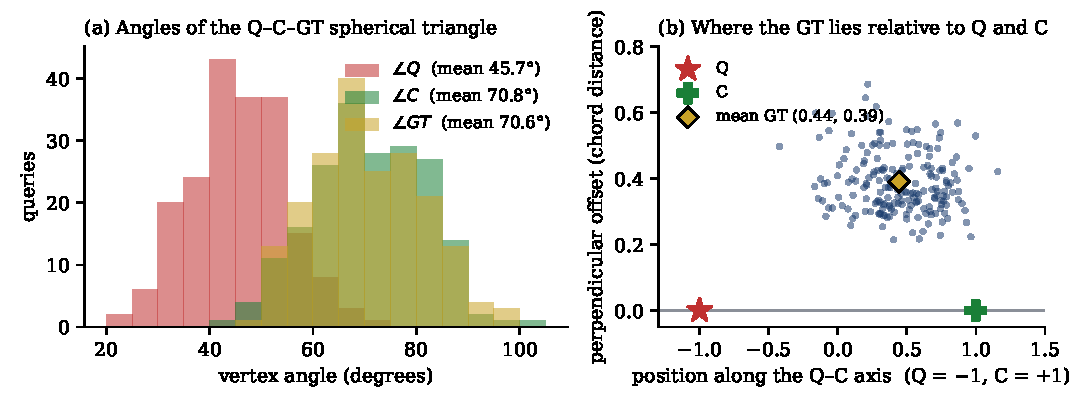
\includegraphics[width=\textwidth]{triangle.pdf}
\caption{The $Q$-$C$-$GT$ triangle over 196 queries. (a) Vertex angles: the apex at $Q$ is sharp and the two base angles are nearly equal. (b) Position of the GT in the $Q$-$C$ frame: it lies on the centroid's side of the midpoint but consistently off the axis.}
\label{fig:triangle}
\end{figure}

\subsubsection{Finding B: relevance is graded geometrically around the GT}

Mean distance to the GT decreases monotonically with the judged relevance of a document: 0.89, 0.84, 0.77, 0.63, 0.40 and 0.22 for scores 0.1, 0.2, 0.4, 0.6, 0.8 and 1.0 (Fig.~\ref{fig:gradient}). The relation holds query by query, not only in aggregate: the Spearman correlation between a document's score and its distance to the GT is negative for all 196 queries (median $-0.29$, range $-0.46$ to $-0.07$, $p<0.05$ in every query; Pearson median $-0.50$). The score identifies the GT with ROC-AUC $=0.9974$: the GT receives a mean score of 0.996 against 0.151 for the other 999,987 judged pairs, and it receives the top score (1.0) in 186 of the 187 queries where it was judged. Two consequences follow. First, the judge is a reliable \emph{instrument}: when it says a document is fully relevant, that document is geometrically close to the GT.

\begin{figure}[H]
\centering
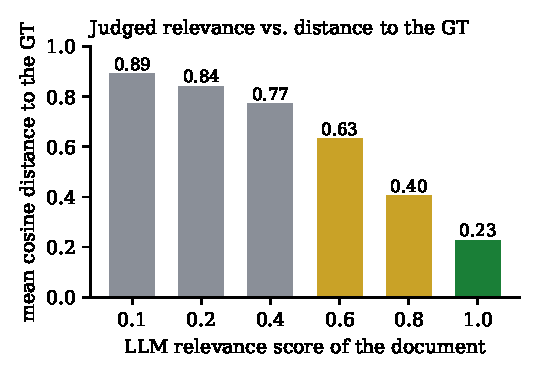
\includegraphics[width=0.55\textwidth]{gradient.pdf}
\caption{Mean cosine distance to the GT of non-GT documents, by LLM relevance score ($\sim$985k judged pairs). The relationship is monotone at every level.}
\label{fig:gradient}
\end{figure}

Second, the judge cannot replace geometry. Table~\ref{tab:rerank} re-ranks B1's top-$k$ purely by judged relevance, the operation an LLM re-ranker performs: top-1 accuracy \emph{falls} from 70.4\% to 40.8\% at $k=5$ and keeps falling as the window widens, even though the GT is inside the window for 88-100\% of queries. The reason is that on average 17 documents per query share the top score and the GT is only one of them. Ranking by relevance alone cannot single out the GT; position in the space can.

\begin{table}[H]
\centering\small
\caption{Re-ranking B1's top-$k$ by the judge's relevance score (ties keep B1 order). The GT is inside the window for the share of queries shown; re-ranking still cannot place it first.}
\label{tab:rerank}
\setstretch{1.05}
\begin{tabular}{lccccc}
\toprule
$k$ & 5 & 10 & 20 & 50 & 100 \\
\midrule
GT inside top-$k$ of B1 & 88.3\% & 91.8\% & 94.9\% & 100\% & 100\% \\
Top-1 after re-ranking  & 40.8\% & 32.1\% & 18.9\% & 11.2\% & 10.2\% \\
Mean GT rank after re-ranking & 2.35 & 3.52 & 7.33 & 10.82 & 13.52 \\
\bottomrule
\end{tabular}
\end{table}

\subsubsection{Finding C: static anchoring heuristics barely help}
\label{sec:prelim-static}

Algorithm~\ref{alg:static} defines the five static strategies compared in Table~\ref{tab:results}; all rank the whole pool once and report the position of the GT. B1 is the standard retriever; B2 is the oracle centroid alone; H1 blends the two distances; H2 uses the centroid only to break ties; H3 re-ranks the top-$k$ of B1 by the centroid.

\begin{algorithm}[H]
\caption{Static anchoring family (Table~\ref{tab:results})}
\label{alg:static}
\begin{algorithmic}[1]
\Require $Q$, pool $\mathcal{D}$, oracle centroid $C$, mode $\in\{$B1, B2, H1($\alpha$), H2, H3($k$)$\}$
\Statex \textbf{B1:} $f(d) \gets \dist(d,Q)$ \qquad \textbf{B2:} $f(d) \gets \dist(d,C)$ \qquad \textbf{H1:} $f(d) \gets \alpha\,\dist(d,Q) + (1-\alpha)\,\dist(d,C)$
\Statex \textbf{H2:} sort by $(\dist(d,Q),\ \dist(d,C))$ lexicographically
\Statex \textbf{H3:} $S \gets$ the $k$ documents with smallest $\dist(d,Q)$;\; rank $S$ by $\dist(d,C)$;\; append $\mathcal{D}\setminus S$ in B1 order
\State \Return rank of $GT$ in the resulting order \Comment{$=$ documents inspected until GT}
\end{algorithmic}
\end{algorithm}

\begin{table}[H]
\centering\small
\caption{GT rank statistics on 196 queries. $\dist(\cdot)$ is cosine distance; $C$ is the oracle centroid.}
\label{tab:results}
\setstretch{1.05}
\begin{tabularx}{\textwidth}{Xcccc}
\toprule
Algorithm & Mean rank & Top-1 (\%) & Top-3 (\%) & Top-10 (\%) \\
\midrule
B1: rank by $\dist(Q)$ (standard RAG)                      & 3.29 & 70.4 & 83.2 & 91.8 \\
B2: rank by $\dist(C)$                                      & 9.87 & 14.8 & 36.2 & 62.8 \\
H1: $0.93\,\dist(Q) + 0.07\,\dist(C)$                           & 3.35 & \textbf{71.4} & 82.7 & 90.8 \\
H2: $\dist(Q)$, ties broken by $\dist(C)$ ($\equiv$ B1) & 3.29 & 70.4 & 83.2 & 91.8 \\
H3: top-10 by $\dist(Q)$, re-ranked by $\dist(C)$               & 5.05 & 17.9 & 43.9 & 91.8 \\
\bottomrule
\end{tabularx}
\end{table}

Figure~\ref{fig:sweeps}(a,b) shows the full parameter sweeps behind the table. H1 peaks at 71.4\% for $\alpha\in[0.90,0.93]$ and falls to 59.7\% at $\alpha=0.51$; H3 is 17.9\% at $k=10$ and converges to B2 (14.8\%) for $k\ge50$. H2 is identical to B1 because 64-bit cosine distances never tie. A small, static pull toward the oracle centroid is therefore worth about one point of top-1; anything stronger hurts. Replacing the query outright is worse still. Table~\ref{tab:prf} reports an iterative, LLM-filtered PRF: inspect B1's top-$k$, build a centroid from those judged above a threshold, re-rank the whole pool by distance to that centroid, and repeat. Every configuration is far below B1, the best being the smallest window with the strictest filter (31.1\% at $k=5$, threshold 1.0), and additional rounds make it worse, because each round re-centers on a cluster that may not contain the GT. The centroid is a correction to the query, not a substitute for it.

\begin{table}[H]
\centering\small
\caption{Iterative LLM-filtered PRF: top-1 accuracy (\%) after re-ranking the pool by the centroid of the top-$k$ documents judged above the threshold, for one to three feedback rounds. B1 is 70.4\%.}
\label{tab:prf}
\setstretch{1.05}
\begin{tabular}{lcccccc}
\toprule
 & \multicolumn{3}{c}{threshold $\geq 0.5$} & \multicolumn{3}{c}{threshold $= 1.0$} \\
\cmidrule(lr){2-4}\cmidrule(lr){5-7}
$k$ & round 1 & round 2 & round 3 & round 1 & round 2 & round 3 \\
\midrule
5  & 24.0 & 13.3 & 12.2 & 31.1 & 24.0 & 23.5 \\
10 & 18.9 & 7.1  & 6.6  & 26.0 & 17.9 & 15.3 \\
20 & 13.8 & 8.7  & 8.7  & 18.9 & 15.3 & 14.8 \\
50 & 13.3 & 11.7 & 11.7 & 16.3 & 16.8 & 16.8 \\
\bottomrule
\end{tabular}
\end{table}

The 58 queries where B1 misses the GT are mostly \emph{soft} failures. The GT is at position 2 in 19 of them, at positions 3-5 in 16, at 6-10 in 7, and beyond 10 in 16. In 46 of the 58 (79\%) the document B1 returns first is itself scored 1.0, in 5 more it is scored 0.8, and only 7 queries return a first document scored 0.6 or less; every failing query has at least one document scored $\geq0.8$ in its top 10. These queries have \emph{more} fully relevant documents than the others (7.5 vs.\ 6.5 in the top 10, 19.9 vs.\ 15.9 in the whole pool), which suggests that many of them have several valid answers and that the label singles out one of them. This is why Algorithm~\ref{alg:adaptive} reports soft and exact success separately, and why the seven hard failures are the first targets of the Phase~1 failure analysis.

\subsubsection{Finding D: a first adaptive prototype, and what it teaches}
\label{sec:prelim-adaptive}

A prototype of adaptive anchoring was implemented as a sequential simulation: inspect documents one at a time, start from pure $\dist(Q)$ order, and as soon as a document is judged 1.0 begin ranking the remaining documents by Eq.~\ref{eq:score} with a \emph{fixed} $\alpha$ and a centroid rebuilt from every 1.0 document found so far. Figure~\ref{fig:sweeps}(c) shows the result: the mean number of documents inspected until the GT rises monotonically from 3.29 at $\alpha=1$ (B1) to 4.55 at $\alpha=0.1$. Naive adaptivity hurts. The reasons are instructive and shape Algorithm~\ref{alg:adaptive}: the centroid is formed from one or two documents and is therefore noisy exactly when it first takes effect; a fixed $\alpha$ applies the same pull whether the centroid rests on one document or ten; the adaptive step is triggered by a \emph{success} (a 1.0 hit) rather than by a failure, so it perturbs queries that B1 was already solving; and with $\sim$17 fully relevant documents per query, pulling toward their centroid moves the anchor toward the cluster but not necessarily toward the GT inside it. The support threshold $m$, the schedule $\alpha(t,|R_t|)$, the failure trigger, and the soft-success criterion in Algorithm~\ref{alg:adaptive} are direct responses to these four observations.

\begin{figure}[H]
\centering
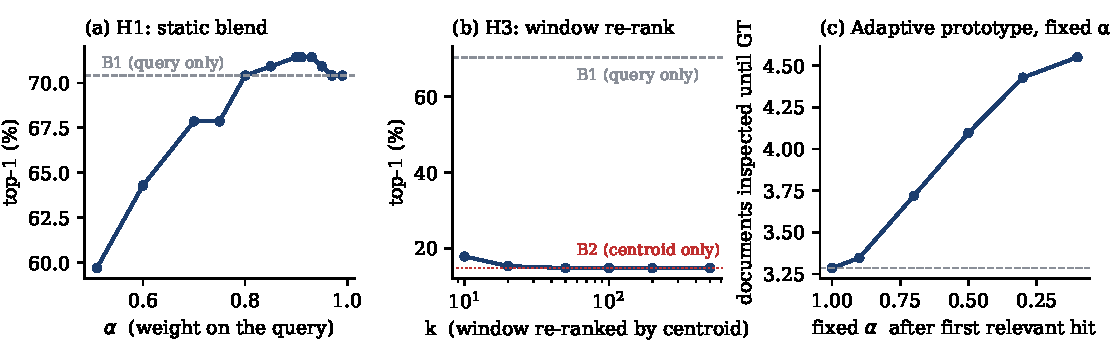
\includegraphics[width=\textwidth]{sweeps.pdf}
\caption{(a) H1 top-1 accuracy as a function of the query weight $\alpha$. (b) H3 top-1 accuracy as a function of the re-ranked window $k$. (c) The adaptive prototype with a fixed $\alpha$: documents inspected until the GT, averaged over 196 queries; $\alpha=1$ is B1.}
\label{fig:sweeps}
\end{figure}

\subsection{Status of the work and plan for the thesis}
\label{sec:thesis}

\textbf{Infrastructure in place.} All experiments above run on one offline framework: a pool in which every query has been judged against every document, cached embeddings, and simulation code in which a ranking policy is a function from pre-computed similarities and judgments to an inspection order. In this framework a new variant of Algorithm~\ref{alg:adaptive} is specified in a few lines and evaluated on all 196 queries in seconds; the static family, the PRF sweeps, the LLM re-ranking study and the adaptive prototype were all produced this way. The same code evaluates the baselines of Section~\ref{sec:anchor-lit} once their update rules are expressed as inspection orders, which they are by construction. Table~\ref{tab:status} maps what exists onto the four research questions.

\begin{table}[H]
\centering\small
\caption{Status of the work by research question.}
\label{tab:status}
\setstretch{1.05}
\begin{tabularx}{\textwidth}{>{\raggedright\arraybackslash}p{3.2cm}>{\raggedright\arraybackslash}X>{\raggedright\arraybackslash}X}
\toprule
 & Done & Remaining \\
\midrule
RQ1 Geometry & Circles, triangle, $Q$-$C$ frame, per-query relevance gradient, extreme-case mechanisms, soft-failure analysis on the biomedical testbed & Failure-prediction model from the geometric features already computed; replication of the measurements on TREC-COVID and MS MARCO using their human judgments \\
RQ2 Anchoring & Static family with full sweeps; iterative PRF; LLM re-ranking; fixed-$\alpha$ adaptive prototype and its diagnosis & Algorithm~\ref{alg:adaptive} (support threshold, schedule, failure trigger, repulsion); the published baselines of Section~\ref{sec:anchor-lit} on the same framework; cost-accuracy curves; soft vs.\ exact success \\
RQ3 Document-space anchor & - & 196 HyDE generations; position in the $Q$-$C$-$GT$ frame; HyDE and ReDE-RF as initial anchors for Algorithm~\ref{alg:adaptive} \\
RQ4 Generalization & - & Phases 1 and 3 on one specialized and one general-domain collection \\
\bottomrule
\end{tabularx}
\end{table}

\textbf{Resources for the remaining phases.} RQ1 and RQ2 need no new data: every variant and every baseline is a ranking policy over the existing similarities and judgments, so the full design space ($\theta$, $m$, schedules, triggers) can be swept exhaustively. RQ3 costs one LLM generation per query. RQ4 reuses public collections that ship with human relevance judgments, so the geometric measurements replicate without LLM judging; where graded judgments are needed to simulate the adaptive search, the volume (a few hundred queries against pools of a few thousand documents) is of the same order as the $\sim$1M pairs already judged once for this testbed, and the judge's reliability on that volume is established by Finding~B.

\textbf{Risks and their mitigations.} Table~\ref{tab:risks} lists the outcomes that could undermine the plan and what each would still yield. The main one is already visible in Finding~D: adaptivity can hurt. Its four causes have concrete remedies built into Algorithm~\ref{alg:adaptive}, and if exact-GT accuracy does not improve, the soft-success analysis still answers a well-defined question - whether a geometrically guided search reaches \emph{a} fully relevant document faster than B1, which is the quantity a RAG system actually consumes.

\begin{table}[H]
\centering\small
\caption{Risks to the plan and the fallback each one leaves.}
\label{tab:risks}
\setstretch{1.05}
\begin{tabularx}{\textwidth}{>{\raggedright\arraybackslash}p{4.4cm}>{\raggedright\arraybackslash}X}
\toprule
Risk & Mitigation / what is still delivered \\
\midrule
Algorithm~\ref{alg:adaptive} does not beat B1 on exact-GT rank & Support threshold, schedule and failure trigger address the diagnosed causes; soft-success and the per-group breakdown (solved vs.\ failed by B1) remain informative; a negative result with a geometric explanation is itself a contribution of RQ1 \\
Published baselines (TOUR, ReDE-RF, BAGEL) already capture the gain & They become the comparison point; the geometric analysis explains \emph{when} each works, which none of them reports \\
HyDE passages are topically right but factually off & This is Hypothesis~D; the $Q$-$C$-$GT$ frame measures it directly, and ReDE-RF-style real-document anchors are the alternative \\
Findings do not transfer to other collections & Phase~1 replication detects this early (S1); the thesis then characterizes the conditions under which the gap appears \\
LLM judge bias in the testbed & Judge reliability is measured (AUC 0.9974, per-query monotonicity); replication collections use human judgments \\
\bottomrule
\end{tabularx}
\end{table}

\textbf{Thesis structure.} (1) Introduction and problem statement; (2) Background - the material of Section~\ref{sec:background}, expanded; (3) The geometry of the query-document space - Findings A-B and the failure-prediction model (RQ1); (4) Geometric anchoring heuristics - Algorithms~\ref{alg:static}-\ref{alg:adaptive}, the published baselines, cost-accuracy results (RQ2); (5) Document-space anchors - HyDE (RQ3); (6) Generalization across collections (RQ4); (7) Conclusions and guidelines. Chapters 2-4 are substantially drafted by the material in this proposal.

\subsection{Time schedule}
Three semesters (Oct 2026 - Mar 2028); the phases overlap because all reuse the existing offline framework.
\begin{table}[H]
\centering\small
\caption{Gantt chart. S1: Oct 2026-Mar 2027; S2: Apr-Sep 2027; S3: Oct 2027-Mar 2028.}
\setstretch{0.95}\setlength{\arrayrulewidth}{0.4pt}
\begin{tabular}{p{7.6cm}|p{1.5cm}|p{1.5cm}|p{1.5cm}|}
\toprule
Phase & \centering S1 & \centering S2 & \centering\arraybackslash S3 \\
\midrule
Literature review and baseline setup        & \cellcolor{bgunavy!55} &   &   \\
Phase 1: geometric analysis and replication & \cellcolor{bgunavy!55} &   &   \\
Phase 2: HyDE evaluation                    & \cellcolor{bgunavy!55} & \cellcolor{bgunavy!55} &   \\
Phase 3: adaptive geometric anchoring       & \cellcolor{bgunavy!55} & \cellcolor{bgunavy!55} &   \\
Phase 4: cross-domain generalization        &   & \cellcolor{bgunavy!55} & \cellcolor{bgunavy!55} \\
Paper writing and submission                &   & \cellcolor{bgunavy!25} & \cellcolor{bgunavy!25} \\
Thesis writing and finalization             &   &   & \cellcolor{bgunavy!25} \\
\bottomrule
\end{tabular}
\end{table}

% ============================================================
% BIBLIOGRAPHY
% ============================================================
\section*{Bibliography}
\renewcommand{\bibsection}{}
\begin{multicols}{2}
\footnotesize\setstretch{0.92}\setlength{\bibsep}{1.5pt}
\bibliographystyle{plainnat-hyphen}
\bibliography{references,refs_rag,refs_geometry,refs_new}
\end{multicols}

\end{document}
